%----------------------------------------------------------------------------------------
%	PACKAGES AND OTHER DOCUMENT CONFIGURATIONS
%----------------------------------------------------------------------------------------

\documentclass[fleqn,10pt]{SelfArx} % Document font size and equations flushed left

%----------------------------------------------------------------------------------------
%	COLUMNS
%----------------------------------------------------------------------------------------

% \setlength{\columnsep}{0.55cm} % Distance between the two columns of text
% \setlength{\fboxrule}{0.75pt} % Width of the border around the abstract

%----------------------------------------------------------------------------------------
%	COLORS
%----------------------------------------------------------------------------------------

\definecolor{color1}{RGB}{0,0,90} % Color of the article title and sections
\definecolor{color2}{RGB}{0,20,20} % Color of the boxes behind the abstract and headings

%----------------------------------------------------------------------------------------
%	HYPERLINKS
%----------------------------------------------------------------------------------------

\usepackage{hyperref} % Required for hyperlinks
\hypersetup{hidelinks,colorlinks,breaklinks=true,urlcolor=color2,citecolor=color1,linkcolor=color1,bookmarksopen=false,pdftitle={Title},pdfauthor={Author}}

%----------------------------------------------------------------------------------------
%	ARTICLE INFORMATION
%----------------------------------------------------------------------------------------

\PaperTitle{Ferramentas de DevOps} % Article title
\JournalInfo{Versão 1.0} % Journal information
\Archive{} % Additional notes (e.g. copyright, DOI, review/research article)

\Authors{Tradução e Adaptação por Fernando Anselmo} % Authors
\affiliation{} % Author affiliation

\Keywords{DevOps --- Ferramentas --- Desenvolvimento} % Keywords - if you don't want any simply remove all the text between the curly brackets
\newcommand{\keywordname}{Keywords} % Defines the keywords heading name

%----------------------------------------------------------------------------------------
%	ABSTRACT
%----------------------------------------------------------------------------------------

\Abstract{Este artigo partiu de uma ideia com base na publicação \textit{50+ Useful DevOps Tools} de \textbf{Agustin Romano} e não é minha intenção tomar a autoria de outra obra. O que fiz neste trabalho foi realizar uma tradução e em muitas oportunidades a complementação de dados faltantes nos assuntos abordados e atualização para a realidade. Nesta versão constam 65 ferramentas divididas em Infraestrutura, Integração e Entrega Contínua, Construção, Bases de Dados e Big Data, Implantação, Testes, Segurança, Monitoramento e Visualização.}

%----------------------------------------------------------------------
% Início do Documento
%----------------------------------------------------------------------
\begin{document}
	
\maketitle % mostrar o título
\thispagestyle{fancy} % habilitar o cabeçalho/rodapé das páginas

\section*{Histórico}

Essa metodologia é considerada uma abordagem para o Gerenciamento de Software, apareceu pela primeira vez em 2009 e passou a significar muitas coisas para cada indivíduo que usa o termo, \textit{DevOps} não é um padrão, software ou processo definido, mas uma cultura. O Gartner define DevOps como: 
\begin{quotation}
	\textit{DevOps represents a change in IT culture, focusing on rapid IT service delivery through the adoption of agile, lean practices in the context of a system-oriented approach. DevOps emphasizes people (and culture), and seeks to improve collaboration between operations and development teams. DevOps implementations utilize technology — especially automation tools that can leverage an increasingly programmable and dynamic infrastructure from a life cycle perspective\footnote{DevOps representa uma mudança de cultura em TI, foco na entrega rápida de serviços por meio da adoção de práticas ágeis e enxutas no contexto em uma Abordagem Orientada a Sistemas. \textit{DevOps} enfatiza as pessoas (e a cultura), busca melhorar a colaboração entre as equipes de operações e desenvolvimento. As implementações de \textit{DevOps} utilizam tecnologia - especialmente ferramentas de automação que podem alavancar uma infraestrutura cada vez mais programável e dinâmica em uma perspectiva voltada ao ciclo de vida.}.}
\end{quotation}

DevOps é uma abordagem multifacetada para o Ciclo de Vida do Desenvolvimento de Software (\textbf{SDLC}), a principal força é como alavanca a tecnologia e o software para agilizar todo o processo. Portanto, a abordagem certa é a adoção das filosofias de cooperação e implementação das ferramentas certas, a empresa pode aumentar a frequência de implantação e os tempos de entrega em relação aos métodos tradicionais.

\subsection*{Lista de Abreviaturas}
Na área de DevOps devemos conhecer vários termos, que normalmente são utilizados como abreviaturas, estes são alguns que trataremos neste artigo, recomendo conhecê-los antes mesmo de ver a relação dos softwares: \begin{itemize}[nolistsep]
	\item AD -- Active Directory
	\item AWS -- Amazon Web Services
	\item BI -- Business Intelligence
	\item Bot -- diminutivo de robot
	\item CaaS -- Containers as a Service
	\item CRON -- Agendador de tarefas
	\item DBMS -- Database Management System
	\item DSL -- Digital Subscriber Line
	\item Gnome HIG -- GNOME Human Interface Guidelines
	\item IaC -- Infrastructure as Code
	\item IDE -- Integrated Development Environment
	\item INI - Initialize - Arquivos texto com estrutura básica composta de seções e propriedades
	\item JSON -- JavaScript Object Notation
	\item LDAP -- Lightweight Directory Access Protocol
	\item MFA -- Multi-Factor Authentication
	\item RDBMS -- Relational Database Management System
	\item SaaS -- Software as a Service
	\item SBT -- Scala Build Tool 
	\item SDLC -- Systems Development Life Cycle
	\item SSH -- Secure Shell
	\item SSO -- Single Sign-On
	\item UX -- User eXperience
	\item YAML -- YAML Ain't Markup Language
\end{itemize}

Esta lista procura ser a mais abrangente possível. Compreende ferramentas bem estabelecidas e os lançamentos mais recentes do mercado - de qualquer forma, é provável que exista uma ferramenta que pode ser um trunfo para seu o negócio. Para aqueles que já vivem e respiram \textit{DevOps}, desejamos que encontrem algo para auxiliá-los em seu crescimento.

\section*{Ciclo Infinito DevOps}
Com tantas opções em ferramentas, não há uma resposta \aspas{certa} para quais devemos adotar? Nenhuma ferramenta cobrirá todas as necessidades e será implantada em uma variedade de equipes operacionais e de desenvolvimento, então analisemos as etapas do processo antes de escolher qual ferramenta pode funcionar:
\begin{figure}[H]
	\centering
	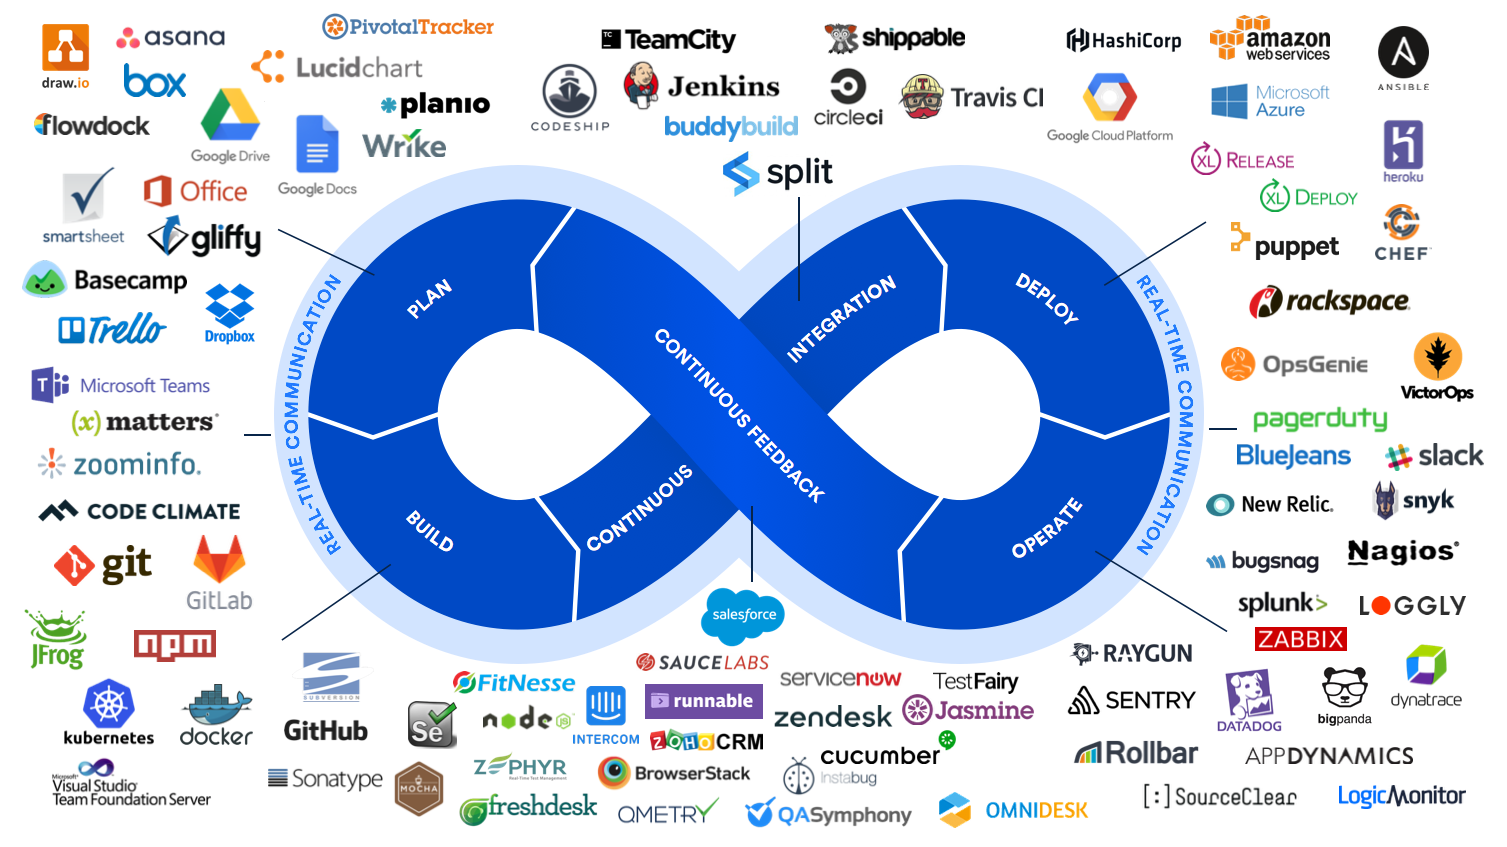
\includegraphics[width=0.8\textwidth]{imagens/devops}
\end{figure}

\begin{itemize}
	\item \textbf{Planejamento}: antes mesmo de começar com \textbf{SDLC}, a empresa precisa ter uma ideia coesa de quais ferramentas precisam implementar em suas equipes. Existem algumas que podem auxiliar nessa primeira etapa crucial.
	\item \textbf{Resposta Contínua}: precisam ser mantidas previsíveis, suaves e confiáveis com riscos mínimos; a automação tem um papel importante nesse processo.
	\item \textbf{Operação e Implantação}: são ferramentas que criam ambientes provisionados de forma idêntica. A última coisa que precisamos ouvir é a frase: \aspas{Mas isso funciona no meu computador}.
	\item \textbf{Integração Contínua}: ferramentas precisam fornecer respostas constantes e imediatas, várias vezes ao dia, mas nem todas as integrações são implementadas da mesma forma. A ferramenta que desejamos selecionar é a certa para o trabalho?
	\item \textbf{Construção}: se tornou rapidamente uma moeda do \textit{DevOps}, mas a automação sempre aumenta drasticamente a produção em relação aos métodos manuais.
\end{itemize}

\section*{Divisão Lógica das Ferramentas}

\subsection*{Infraestrutura}

\textbf{Docker} \\
É um pacote de tecnologia DevOps. Permite que as equipes criem, enviem e executem aplicativos distribuídos e que os usuários combinem esses aplicativos através de componentes que trabalham juntos. Quando o \textbf{CaaS} está pronto, é uma plataforma que trabalha com orquestração. Suporte integrado para \textbf{Google Cloud} e \textbf{AWS}. Aplicativos novos e existentes são suportados e oferece uma plataforma de contêiner pronta para organização, independentes de plataforma em ambientes de máquina virtual.

Link: \url{https://www.docker.com/}

\textbf{AWS CloudFormation} \\
É uma necessidade absoluta se atualmente estamos trabalhando ou planejando ir para a nuvem AWS. Permite modelar a infraestrutura AWS e provisionar os recursos de forma rápida e fácil. Tudo isso é feito em um arquivo padrão \textbf{JSON} ou \textbf{YAML} e o serviço possui uma variedade de recursos para automação, e garante que as implantações sejam previsíveis, confiáveis e gerenciáveis.

Link: \url{https://aws.amazon.com/cloudformation/URL}

\textbf{Azure Resource Manager} \\
ARM é a resposta da Microsoft para uma ferramenta IaC abrangente. Com seus modelos descritos em arquivos padrão \textbf{JSON}, o \textit{Azure Resource Manager} provisiona a infraestrutura, lida com dependências e declara vários recursos por meio de um único modelo.

Link: \url{https://azure.microsoft.com/en-us/features/resource-manager/}

\textbf{Google Cloud Deployment Manager} \\
Outra ferramenta IaC agora da \textit{Google} para \textit{Google Cloud Platform}. Esta ferramenta utiliza padrão \textbf{YAML} para os arquivos de configuração e \textbf{Jinja2} ou \textbf{Python} para os modelos. Alguns de seus recursos notáveis são a implantação síncrona e visualização, isso permite uma visão geral das mudanças antes de serem confirmadas.

Link: \url{https://cloud.google.com/deployment-manager/}

\textbf{DigitalOcean} \\
Provedor de hospedagem na nuvem e possui um rápido crescimento. Em segundos, pode implantar uma máquina virtual baseada em Linux - conhecida como ‘Droplet’. Apresenta alta confiabilidade em relação a porcentagem do tempo de atividade e tempos médios de carregamento.

Link: \url{https://www.digitalocean.com/}

\textbf{Terraform} \\
É muito diferente das ferramentas mencionadas acima, pois não está restrito a um ambiente de nuvem específico, o que traz maiores benefícios para lidar com aplicativos distribuídos complexos sem estar vinculado a uma única plataforma. E assim como o \textit{Google Cloud Deployment Manager}, também possui recurso de visualização.

Link: \url{Link: https://www.terraform.io/}

\textbf{Chef} \\
Uma escolha ideal para quem gosta de CI/CD. Em essência utiliza receitas, modelos e \textit{cookbooks} (livros de receitas) no qual descrevemos as ações necessárias para a execução dos serviços. Possui uma coleção extensa de modelos prontos. Os \textit{cookbooks} permitem uma configuração consistente, mesmo quando a infraestrutura aumenta rapidamente. Tudo isso está embrulhado em um padrão \textbf{DSL} com base em \textbf{Ruby}.
Link: \url{https://www.chef.io/products/chef-infra/}

\textbf{Ansible} \\
Uma das melhores ferramentas quando tratamos de automatizar tarefas repetitivas, como gerenciamento de configuração, implantação de aplicativos e orquestração intra-serviço. Sem infraestrutura de segurança personalizada adicional e sem agentes, é fácil de implantar e executar com arquivos padrão \textbf{YAML}, permite descrever a automação de uma forma que se aproxima de um texto básico em inglês.

Link: \url{https://www.ansible.com/}

\textbf{Puppet} \\
Talvez seja a ferramenta IaC mais antiga desta lista, e com isso vem muita experiência e maturidade em seu campo através de uma comunidade bem movimentada. O que diferencia esta ferramenta é sua abordagem para configuração e automação, pois precisamos definir um estado declarativo, e esta se encarregará em descobrir a melhor forma de atingir esse estado.

Link: \url{https://puppet.com/}

\textbf{Rudder} \\
Destinada a configuração e supervisão contínuas. Oferece várias opções, como usuários não especialistas, especialistas e administradores, além de automatizar tarefas comuns para o gerenciamento do sistema, como instalação e configuração.

Link: \url{https://www.rudder.io/}

\subsection*{Integração e Entrega Contínua}

\textbf{Jenkins} \\
É um servidor de automação \textit{open source}. Ajuda a automatizar as partes do desenvolvimento de software relacionadas à construção, teste e implantação, facilita a integração e entrega contínuas. É um sistema baseado em servidor que é executado em contêineres \textit{Servlet} como o \textbf{Apache Tomcat}. Suporta ferramentas para controle de versão e pode executar \textbf{Apache Ant}, \textbf{Apache Maven} e projetos baseados em \textbf{SBT}, bem como \textit{scripts} de \textit{shell} e comandos em lote do Windows ou Linux. Os builds podem ser acionados por vários meios, por exemplo, pela confirmação de um \textit{commit}, agendamento por meio de um mecanismo semelhante ao \textbf{CRON}. Também pode ser acionado após a conclusão de outras compilações na fila.

Link: \url{https://www.jenkins.io/}

\textbf{Pagerduty} \\
Auxilia as empresas aumentar a reputação da marca. É uma solução para o gerenciamento de eventos que apoia a estratégia de entrega contínua. Permite que as equipes forneçam aplicativos de alto desempenho. Mecanismo de alerta confiável que fornece resultado em tempo real. Agrupamento de atividades e visibilidade em sistemas e aplicativos.Auxilia a identificar e resolver facilmente eventos do desenvolvimento à produção e um sistema de colaboração em tempo real com relatórios de usuários.

Link: \url{https://www.pagerduty.com/}

\textbf{CircleCI} \\
Destinada a processos de implantação abrangentes e fornece uma plataforma de ponta para integração e entrega e busca liberar seu código em todo o mundo por meio de automação, construção e teste.

Link: \url{https://circleci.com/}

\textbf{Harness} \\
Uma das primeiras plataformas de entrega contínua como serviço, auxilia as equipes de implantação a automatizar todo o processo de entrega contínua e a fornecer segurança quando as implantações falham.

Link: \url{Link: https://harness.io/}

\textbf{Buddy} \\
Com uma interface \textbf{UX} (usabilidade para o usuário final) simples, o é uma ferramenta inteligente de CI/CD que reduz bastante o limite de entrada para DevOps.

Link: \url{Link: https://buddy.works/}

\subsection*{Construção}

\textbf{Gulp} \\
Automatiza a difícil tarefa do processo de desenvolvimento para o kit de ferramentas \textbf{Javascript}. É fácil de usar e oferece simples \textit{plugins} para trabalhar de acordo com os requisitos e cria arquivos finais de modo mais rápido, não gerando gravações desnecessárias no disco.

Link: \url{https://gulpjs.com/}

\textbf{Probot} \\
Fornece uma estrutura de "robôs" (\textbf{bot}) para a criação de aplicativos que é otimizada pelo \textbf{GitHub}. Esses robôs são fáceis de escrever, implantar e compartilhar.

Link: \url{https://probot.github.io/}

\textbf{AWS Opsworks} \\
Destinada para aqueles que utilizam o \textit{Chef Automate} e o \textit{Puppet Enterprise} na AWS. Podemos automatizar facilmente como os servidores são implantados, configurados e gerenciados.

Link: \url{https://aws.amazon.com/opsworks/}

\textbf{Relay} \\
Arquiteturas Orientadas a Eventos certamente não é uma ideia nova, mas esta ferramenta foi projetada especificamente com DevOps em mente. Possui uma quantidade impressionante de integrações e fluxos de trabalho para uso imediato, vital para automatizar tarefas de baixo valor para que possamos nos concentrar no que é mais importante para a equipe.

Link: \url{https://relay.sh/}

\textbf{CA Automic Workload Automation} \\
Este é um guia abrangente sobre tudo no qual o \textbf{CA Automic} oferece quando se trata do plano para automação das cargas de trabalho.

Link: \url{https://docs.automic.com/documentation}

\subsection*{Bases de Dados e Big Data}

\textbf{MySQL} \\
É um \textbf{RDBMS} relativamente fácil de usar, muitos não sabem mas é utilizado para armazenar grandes quantidades de informações e considerado como uma solução estável, confiável e poderosa com recursos avançados. Tem sido usado por grandes corporações da indústria como Facebook, NASA, Paypal e Google.

Link: \url{https://www.mysql.com/}

\textbf{MariaDB} \\
É um \textbf{RDBMS} \textit{open source} criado pelos desenvolvedores a partir do MySQL. Alguns de seus usuários são Wikipedia, WordPress.com e Google. É uma boa escolha para um servidor rápido, escalonável e robusto.

Link: \url{https://mariadb.org/}

\textbf{Liquibase} \\
Outra ferramenta de \textit{open source} para Bancos de Dados que lidam com mudanças e gerenciamento de implantação. Também ajuda as equipes no controlar da versão do banco de dados, implantação do esquema e as mudanças lógicas.

Link: \url{https://www.liquibase.org/}

\textbf{Looker} \\
Parte do \textbf{Google Cloud}, é uma plataforma de BI (\textit{Business Intelligence}) e análise de dados altamente adaptável que se integra perfeitamente com \textbf{Redshift}, \textbf{Snowflake}, \textbf{BigQuery} e mais de 50 dialetos SQL.

Link: \url{https://looker.com/}

\textbf{Apache Hadoop} \\
Projetado para ser facilmente escalonável, sua estrutura permite que grandes conjuntos de dados sejam distribuídos em um único servidor ou em milhares de computadores. Possui uma biblioteca projetada para implementar computação e armazenamento em nível local.

Link: \url{https://hadoop.apache.org/}

\textbf{HPCC Systems} \\
Conta com duas décadas de experiência na indústria de dados para trazer uma plataforma de \textit{Data Lake} de ponta a ponta e \textit{open source}.

Link: \url{https://hpccsystems.com/}

\textbf{BigQuery} \\
Fornecido pelo \textbf{Google}, é a resposta ao mecanismo de pesquisa para obter \textit{Data Warehouses} escalonáveis, econômicos e sem servidor para as massas.

Link: \url{https://cloud.google.com/bigquery}

\textbf{Apache Cassandra} \\
É um projeto para \textbf{DBMS} distribuídos altamente escalável e de segunda geração. A ferramenta ideal quando se trata de dados críticos, com sua tolerância a falhas comprovada e escalabilidade linear, garante que o banco de dados sempre manterá um alto nível de escalabilidade e disponibilidade.

Link: \url{https://cassandra.apache.org/}

\textbf{MongoDB} \\
DBMS orientado a documentos livre, \textit{open source} e multiplataforma, escrito na linguagem C++. Classificado como um banco de dados padrão NoSQL, possui uma abordagem única na forma de armazenar os dados, através de documentos padrão \textbf{JSON}, o que cria um sistema incrivelmente flexível, escalonável e dinâmico.

Link: \url{https://www.mongodb.com/}

\textbf{Qlik} \\
Duas ferramentas fazem parte do conjunto QlikSense e QlikView, os dados brutos são altamente acionáveis através da abordagem de ponta a ponta para integração e análise de dados para maximizar a transformação dos dados em percepções a partir das quais o negócio pode crescer.

Link: \url{https://www.qlik.com/}

\textbf{Sisense} \\
é uma força motriz por trás da construção e implementação de aplicativos analíticos. A plataforma de dados e análise oferece um sistema ágil de \textbf{BI} voltado para transformar dados simples em ferramentas analíticas poderosas.

Link: \url{https://www.sisense.com/}

\textbf{Talend} \\
Entrou em 2005 e foi a primeira fornecedora de um software comercial \textit{open source} para integração de dados e ainda é uma concorrente líder em seu campo. É uma plataforma de integração que auxilia na transformação dos dados em percepções de negócios. 

Link: \url{https://www.talend.com/}

\subsection*{Implantação}

\textbf{Awless} \\
Uma interface para \textbf{CLI} que visa ajudar os desenvolvedores a gerenciar o \textit{Amazon Web Services}. Sincroniza de forma transparente com um gráfico local representacional do recurso da nuvem e seu relacionamento.

Link: \url{Link: https://github.com/wallix/awless}

\textbf{Snyk-CLI} \\
Auxilia na descoberta e, mais importante, a corrigir vulnerabilidades em dependências, tanto em uma rede quanto em sistemas de \textbf{CI}.

Link: \url{https://support.snyk.io/hc/en-us}

\textbf{Daytona} \\
Auxilia através de uma versão mais simplificada da \textbf{CLI} do cliente \textbf{Vault} com um foco especial na autenticação automatizada e na busca de segredos.

Link: \url{https://github.com/cruise-automation/daytona}

\textbf{Bitbucket} \\
Para equipes onde o planejamento de projetos, colaboração em código, teste e implantação podem acontecer em um único lugar com opções de assinatura gratuita ou paga.

Link: \url{https://bitbucket.org/product}

\textbf{Confluence} \\
Perfeita para planejamento de projetos e marketing, notas de reuniões e postagem em blogs. Cria um espaço de trabalho aberto e é acessível para o negócio.

Link: \url{https://www.atlassian.com/software/confluence}

\textbf{Frame.ai} \\
Assume uma postura única nas relações com o cliente e ajuda a identificar o "por quê?" Por trás dos resultados do cliente por meio de recursos para o monitoramento contínuo.

Link: \url{https://frame.ai/}

\textbf{Grit} \\
Ferramenta do GitHub que auxilia os programadores/desenvolvedores a armazenar, transferir, compartilhar e copiar \textit{commits} de um repositório origem para um de destino. A intenção é espelhar projetos que residem em um repositório particular para um Git externo específico do projeto.

Link: \url{https://github.com/grailbio/grit}

\textbf{JIRA} \\
Auxilia os desenvolvedores a capturar, atribuir e definir prioridades em uma tarefa pretendida. Permite que o desenvolvedor gerencie todo o processo de desenvolvimento do sistema garantindo que todas as tarefas sejam concluídas.

Link: \url{https://www.atlassian.com/software/jira}

\textbf{EditorConfig} \\
Voltada aos desenvolvedores que trabalham em grandes grupos com diferentes editores de texto ou \textbf{IDEs} a manter estilos de codificação consistentes.

Link: \url{https://editorconfig.org/}

\textbf{Tilix} \\
Emulador de terminal para Linux que segue \textbf{Gnome HIG}. Basicamente é um emulador de terminal com o recurso de \textit{tile}, ou \textit{split}, que permite a divisão da tela em várias colunas e linhas e facilita a execução de diversas tarefas na mesma janela.

Link: \url{https://gnunn1.github.io/tilix-web/}

\textbf{Jsonnet} \\
Facilita o entendimento de arquivos tipo \textbf{JSON}. A ferramenta apresenta uma variedade de recursos, como eliminação de duplicação, integração com aplicativos personalizados / existentes e pode gerar outros formatos, que inclui \textbf{INI} e \textbf{YAML}.

Link: \url{https://jsonnet.org/}

\textbf{Hazelcast} \\
Solução de cache em memória que oferece aplicativos, de baixa latência e centrados em dados. Pode acomodar o processamento em tempo real de qualquer aplicativo com arquitetura multi-serviço de processamento paralelo.

Link: \url{https://hazelcast.com/}

\textbf{Vagrant} \\
Criação e gerenciamento de ambientes em máquina virtual através de um único fluxo de trabalho. Oferece um ambiente fácil de usar e se concentra na automação. Reduz o tempo de instalação e melhora a qualidade do produto se integra às ferramentas para gerenciamento de configuração existentes, tais como \textbf{Chef}, \textbf{Puppet}, \textbf{Ansible} e \textbf{Salt}. Funciona perfeitamente nos sistemas operacionais macOS, Linux, Windows. Auxilia que a equipe DevOps tenha um ambiente de desenvolvimento ideal.

Link: \url{https://www.vagrantup.com/}

\subsection*{Testes}

\textbf{Selenium} \\
\textit{Open source} para gerenciar e executar roteiros de testes automatizados para aplicativos da Web e \textit{Desktop}. Possui uma interface fácil para desenvolver testes automatizados. Permite a regressão baseada em navegador é ideal para criar suítes e testes de automação com \textit{scripts} de teste em várias linguagens, tais como Java, Python, Ruby, C\#, Perl, Php, JavaScript. Suporta Multiplataformas como IOS e Android.

Link: \url{https://www.selenium.dev/}

\textbf{CloudEndure} \\
Fornece uma replicação em nível de bloco em tempo real, garante uma melhor integridade de dados com objetivo do ponto de recuperação em segundos para \textbf{DBMS} e aplicativos. O algoritmo de replicação não afeta o desempenho do sistema e nem requer sua reinicialização.

Link: \url{https://www.cloudendure.com/}

\textbf{JMeter} \\
\textit{Open source} desenvolvido com linguagem Java e projetado para testar o comportamento funcional de carga\footnote{O teste de carga permite testar o comportamento de um aplicativo em condições reais, com as solicitações de usuário simultâneas. Isso pode ajudar a determinar o comportamento de um aplicativo quando vários usuários o acessam simultaneamente.} e medir o desempenho. Foi originalmente projetado para testar aplicativos da Web, mas desde então foi expandido para outras funções de teste.

Link: \url{https://jmeter.apache.org/}

\textbf{Vegeta} \\
\textit{Open source} para teste de carga \textbf{HTTP} adaptável que pode ser usada como um utilitário \textbf{CLI} ou uma biblioteca,  escrito na linguagem de programação Go, para executar testes de carga em um aplicativo.

Link: \url{https://github.com/tsenart/vegeta}

\textbf{QuerySurge} \\
Possui o foco em automatizar a validação e o teste dos dados. Alguns recursos são o suporte de plataforma cruzada e com a maioria das soluções voltadas para integração de dados e testes de \textbf{BI}.

Link: \url{Link: https://www.querysurge.com/}

\subsection*{Segurança}

\textbf{WhiteSource Bolt} \\
\textit{Open source} de segurança gratuito para encontrar e corrigir vulnerabilidades no ambiente \textbf{GitHub} ou \textbf{Azure DevOps}. Fornece alertas em tempo real sobre vulnerabilidades conhecidas e auxilia na correção rápida através de sugestões. Suporta mais de 200 linguagens de programação e gerenciadores de pacotes, monitora vários bancos de dados e recomendações de segurança adicionais.

Link: \url{https://bolt.whitesourcesoftware.com/}

\textbf{Krypton} \\
aplicativo móvel autenticador U2F com arquitetura criptografada não \textit{un-phishable} (evitar ataques de phishing). Todas as chaves da criptografia de dados são armazenadas no armazenamento local do dispositivo para evitar acesso externo indesejado.

Link: \url{https://krypt.co/}

\textbf{Mysterium.network} \\
É uma rede de nós que fornece privacidade e segurança aos usuários finais. Esta imagem de nó é criada para hardware de sistema embarcado, como \textbf{Raspberry Pi}.

Link: \url{Link: https://mysterium.network/}

\textbf{Snort} \\
\textit{Open source} que auxilia a identificar intrusos. Expõe ataques maliciosos ao sistema e permite análises de tráfego em tempo real e registros de pacotes. Executa análise de protocolo e pesquisa de conteúdo. Detecção da intrusão com base em assinatura e análise de pacotes, tráfego em tempo real e registro de pacotes. Detecta muitas funções, como estouros de \textit{buffer}, varreduras de portas ocultas e tentativas de impressão digital do sistema operacional.

Link: \url{Link: https://www.snort.org/}

\textbf{Okta} \\
Serviço para gerenciamento de identidade. É possível controlar o acesso dos usuário em único lugar. Os recursos incluem \textbf{SSO}, integração ao \textbf{AD}, \textbf{LDAP} e \textbf{MFA}.

Link: \url{https://www.okta.com/}

\textbf{Smallstep SSH} \\
Fornece acesso \textbf{SSH} de logon único (SSO SSH), um sistema que evita ter de reunir, enviar e girar chaves \textbf{SSH} todos os dias. Esses acessos \textbf{SSH} e sudo podem ser gerenciados por meio de um único painel de administração.
Link: \url{https://smallstep.com/sso-ssh/}

\subsection*{Monitoramento}

\textbf{Prometheus} \\
\textit{Open source} de monitoramento para serviço. Oferece suporte para mais de 10 idiomas e uma linguagem de consulta flexível utilizada para dividir os dados de série temporal coletados para criar tabelas, gráficos e alertas, armazena séries temporais na memória ou disco local, fluxos de valores com registro de data e hora da mesma métrica e o mesmo conjunto de dimensões marcadas. Possui bibliotecas especiais de fácil aplicação.

Link: \url{https://prometheus.io/}

\textbf{Datadog} \\
Serviço de monitoramento para aplicativos em escala de nuvem bem como servidores, bancos de dados, ferramentas e serviços por meio de uma plataforma para análise dos dados baseada em \textbf{SaaS}. Permite coletar todos os metadados não utilizados e que tornam os programas lentos, como consultas ao banco de dados, exceções lançadas, registros de erros não gerenciados e perdas de cache e serviços crescentes. Todos esses eventos, estados de serviço e métricas são coletados em um único lugar e uma representação gráfica visual útil é criada.

Link: \url{https://www.datadoghq.com/}

\textbf{Monit} \\
\textit{Open source} projetado para gerenciar e monitorar sistemas \textbf{UNIX}. Realiza manutenções automáticas e reparos em caso de erros. Executa ações causais significativas em situações de erro. Auxilia a rastrear , arquivos, diretórios e sistemas de arquivos no Localhost, operações \textit{daemon} ou programas semelhantes em execução no host local e fornece conexões de rede para vários servidores.

Link: \url{https://mmonit.com/}

\textbf{M3} \\
Criado pela \textbf{Uber Engineering}, abriga métricas de grande escala que tem sido utilizadas pelo Uber por vários anos e perceberam que as ideias existentes não atendiam aos seus critérios. Foi projetado para maximizar todos os aspectos do pipeline de métricas enquanto minimiza a pegada de hardware.

Link: \url{https://eng.uber.com/m3/}

\textbf{Ganglia} \\
\textit{Open source} de monitoramento distribuído escalonável para sistemas com computação de alto desempenho, como \textit{clusters} e \textit{grids}. Com base em um projeto hierárquico voltado para federações de \textit{clusters} alcança custos indiretos por nó baixo para alta simultaneidade.

Link: \url{http://ganglia.info/}

\textbf{Sensu} \\
Oferece monitoramento multi-nuvem abrangente, de um único servidor para a nuvem. Se integra à várias plataformas usuais e oferece uma forte segurança com os provedores de \textbf{SSO}.

Link: \url{https://sensu.io/}

\textbf{SolarWinds Server and Application Monitor} \\
Monitoramento abrangente e simplificado de aplicativos e servidores. Utilizado para encontrar e resolver problemas de aplicativos antes que se tornem incidentes. Destinado a qualquer aplicativo, servidor e lugar seja sistemas locais, em nuvem ou híbridos. Monitora o desempenho, capacidade e integridade de aplicativos Linux e Windows em \textit{Data Centers}, escritórios remotos e na nuvem.

Link: \url{https://www.solarwinds.com/server-application-monitor}

\subsection*{Visualização}

\textbf{Cloudcraft} \\
Designer visual que ajuda os desenvolvedores a criar diagramas de arquitetura em minutos com componentes inteligentes otimizados para \textbf{AWS}. Elimina a necessidade de desenvolver documentação e especificações estáticas manuais.

Link: \url{https://cloudcraft.co/}

\textbf{DbSchema} \\
Designer para \textbf{DBMS} visual e fácil de usar para gerenciar o esquema do Banco de Dados. Oferece suporte a \textbf{DBMS} padrão \textbf{SQL} e \textbf{NoSQL}

Link: \url{https://dbschema.com/}

\textbf{Juju} \\
Open Source para modelagem de aplicativos. Distribui, configura, dimensiona e executa software para o público e para a nuvem. É possível automatizar a infraestrutura em nuvem e usar arquiteturas de aplicativos. Os administradores podem gerenciar facilmente configuração, manutenção, implantação e escalabilidade em uma poderosa \textbf{GUI} ou interface \textbf{CLI}. Implanta os serviços no ambiente de nuvem em questão de segundos e mantém registros detalhados para resolver problemas rapidamente.

Link: \url{https://jaas.ai/}

\section*{Conclusão}

DevOps é um processo de desenvolvimento e distribuição de software que enfatiza a colaboração e comunicação entre gerenciamento de produtos, desenvolvimento de software e especialistas em operações. Garante que os processos sejam coordenados de maneira ideal.

Sou um entusiasta do mundo \textbf{Open Source} e novas tecnologias. Qual a diferença entre Livre e Open Source? \underline{Livre} significa que esta apostila é gratuita e pode ser compartilhada a vontade. \underline{Open Source} além de livre todos os arquivos que permitem a geração desta (chamados de arquivos fontes) devem ser disponibilizados para que qualquer pessoa possa modificar ao seu prazer, gerar novas, complementar ou fazer o que quiser. Os fontes da apostila (que foi produzida com o LaTex) está disponibilizado no GitHub \cite{github}. Veja ainda outros artigos que publico sobre tecnologia através do meu Blog Oficial \cite{fernandoanselmo}.

%--------------------------------------------------------------------------
% REFERÊNCIAS
%--------------------------------------------------------------------------
\begin{thebibliography}{4}
	\bibitem{artigoOriginal} 
	Artigo Original de Agustin Romano \\
	\url{https://caylent.com/50devops-tools}
	
		\bibitem{fernandoanselmo} 
	Fernando Anselmo - Blog Oficial de Tecnologia \\
	\url{http://www.fernandoanselmo.blogspot.com.br/}
	
	\bibitem{publicacao} 
	Encontre essa e outras publicações em \\
	\url{https://cetrex.academia.edu/FernandoAnselmo}
	
	\bibitem{github} 
	Repositório para os fontes da apostila \\
	\url{https://github.com/fernandoans/publicacoes}
\end{thebibliography}

\end{document}